% GNUPLOT: LaTeX picture with Postscript
\begingroup
  \makeatletter
  \providecommand\color[2][]{%
    \GenericError{(gnuplot) \space\space\space\@spaces}{%
      Package color not loaded in conjunction with
      terminal option `colourtext'%
    }{See the gnuplot documentation for explanation.%
    }{Either use 'blacktext' in gnuplot or load the package
      color.sty in LaTeX.}%
    \renewcommand\color[2][]{}%
  }%
  \providecommand\includegraphics[2][]{%
    \GenericError{(gnuplot) \space\space\space\@spaces}{%
      Package graphicx or graphics not loaded%
    }{See the gnuplot documentation for explanation.%
    }{The gnuplot epslatex terminal needs graphicx.sty or graphics.sty.}%
    \renewcommand\includegraphics[2][]{}%
  }%
  \providecommand\rotatebox[2]{#2}%
  \@ifundefined{ifGPcolor}{%
    \newif\ifGPcolor
    \GPcolortrue
  }{}%
  \@ifundefined{ifGPblacktext}{%
    \newif\ifGPblacktext
    \GPblacktexttrue
  }{}%
  % define a \g@addto@macro without @ in the name:
  \let\gplgaddtomacro\g@addto@macro
  % define empty templates for all commands taking text:
  \gdef\gplbacktext{}%
  \gdef\gplfronttext{}%
  \makeatother
  \ifGPblacktext
    % no textcolor at all
    \def\colorrgb#1{}%
    \def\colorgray#1{}%
  \else
    % gray or color?
    \ifGPcolor
      \def\colorrgb#1{\color[rgb]{#1}}%
      \def\colorgray#1{\color[gray]{#1}}%
      \expandafter\def\csname LTw\endcsname{\color{white}}%
      \expandafter\def\csname LTb\endcsname{\color{black}}%
      \expandafter\def\csname LTa\endcsname{\color{black}}%
      \expandafter\def\csname LT0\endcsname{\color[rgb]{1,0,0}}%
      \expandafter\def\csname LT1\endcsname{\color[rgb]{0,1,0}}%
      \expandafter\def\csname LT2\endcsname{\color[rgb]{0,0,1}}%
      \expandafter\def\csname LT3\endcsname{\color[rgb]{1,0,1}}%
      \expandafter\def\csname LT4\endcsname{\color[rgb]{0,1,1}}%
      \expandafter\def\csname LT5\endcsname{\color[rgb]{1,1,0}}%
      \expandafter\def\csname LT6\endcsname{\color[rgb]{0,0,0}}%
      \expandafter\def\csname LT7\endcsname{\color[rgb]{1,0.3,0}}%
      \expandafter\def\csname LT8\endcsname{\color[rgb]{0.5,0.5,0.5}}%
    \else
      % gray
      \def\colorrgb#1{\color{black}}%
      \def\colorgray#1{\color[gray]{#1}}%
      \expandafter\def\csname LTw\endcsname{\color{white}}%
      \expandafter\def\csname LTb\endcsname{\color{black}}%
      \expandafter\def\csname LTa\endcsname{\color{black}}%
      \expandafter\def\csname LT0\endcsname{\color{black}}%
      \expandafter\def\csname LT1\endcsname{\color{black}}%
      \expandafter\def\csname LT2\endcsname{\color{black}}%
      \expandafter\def\csname LT3\endcsname{\color{black}}%
      \expandafter\def\csname LT4\endcsname{\color{black}}%
      \expandafter\def\csname LT5\endcsname{\color{black}}%
      \expandafter\def\csname LT6\endcsname{\color{black}}%
      \expandafter\def\csname LT7\endcsname{\color{black}}%
      \expandafter\def\csname LT8\endcsname{\color{black}}%
    \fi
  \fi
  \setlength{\unitlength}{0.0500bp}%
  \begin{picture}(12960.00,5760.00)%
    \gplgaddtomacro\gplbacktext{%
      \colorrgb{0.00,0.00,0.00}%
      \put(1552,634){\makebox(0,0)[r]{\strut{}0}}%
      \colorrgb{0.00,0.00,0.00}%
      \put(1552,1807){\makebox(0,0)[r]{\strut{}5}}%
      \colorrgb{0.00,0.00,0.00}%
      \put(1552,2981){\makebox(0,0)[r]{\strut{}10}}%
      \colorrgb{0.00,0.00,0.00}%
      \put(1552,4154){\makebox(0,0)[r]{\strut{}15}}%
      \colorrgb{0.00,0.00,0.00}%
      \put(1552,5327){\makebox(0,0)[r]{\strut{}20}}%
      \colorrgb{0.00,0.00,0.00}%
      \put(1684,414){\makebox(0,0){\strut{}    1}}%
      \colorrgb{0.00,0.00,0.00}%
      \put(2312,414){\makebox(0,0){\strut{}    2}}%
      \colorrgb{0.00,0.00,0.00}%
      \put(2940,414){\makebox(0,0){\strut{}    4}}%
      \colorrgb{0.00,0.00,0.00}%
      \put(3567,414){\makebox(0,0){\strut{}    8}}%
      \colorrgb{0.00,0.00,0.00}%
      \put(4195,414){\makebox(0,0){\strut{}   16}}%
      \colorrgb{0.00,0.00,0.00}%
      \put(4823,414){\makebox(0,0){\strut{}   32}}%
      \colorrgb{0.00,0.00,0.00}%
      \put(5451,414){\makebox(0,0){\strut{}   64}}%
      \colorrgb{0.00,0.00,0.00}%
      \put(6078,414){\makebox(0,0){\strut{}  128}}%
      \colorrgb{0.00,0.00,0.00}%
      \put(6706,414){\makebox(0,0){\strut{}  256}}%
      \colorrgb{0.00,0.00,0.00}%
      \put(7334,414){\makebox(0,0){\strut{}  512}}%
      \colorrgb{0.00,0.00,0.00}%
      \put(7962,414){\makebox(0,0){\strut{} 1024}}%
      \colorrgb{0.00,0.00,0.00}%
      \put(8589,414){\makebox(0,0){\strut{} 2048}}%
      \colorrgb{0.00,0.00,0.00}%
      \put(9217,414){\makebox(0,0){\strut{} 4096}}%
      \colorrgb{0.00,0.00,0.00}%
      \put(9845,414){\makebox(0,0){\strut{} 8192}}%
      \colorrgb{0.00,0.00,0.00}%
      \put(10473,414){\makebox(0,0){\strut{}16384}}%
      \colorrgb{0.00,0.00,0.00}%
      \put(11100,414){\makebox(0,0){\strut{}32768}}%
      \colorrgb{0.00,0.00,0.00}%
      \put(11728,414){\makebox(0,0){\strut{}65536}}%
      \colorrgb{0.00,0.00,0.00}%
      \put(1046,2980){\rotatebox{90}{\makebox(0,0){\strut{}Speedup}}}%
      \colorrgb{0.00,0.00,0.00}%
      \put(6706,84){\makebox(0,0){\strut{}Number of processors}}%
    }%
    \gplgaddtomacro\gplfronttext{%
      \csname LTb\endcsname%
      \put(10741,5154){\makebox(0,0)[r]{\strut{}50\%}}%
      \csname LTb\endcsname%
      \put(10741,4934){\makebox(0,0)[r]{\strut{}75\%}}%
      \csname LTb\endcsname%
      \put(10741,4714){\makebox(0,0)[r]{\strut{}90\%}}%
      \csname LTb\endcsname%
      \put(10741,4494){\makebox(0,0)[r]{\strut{}95\%}}%
    }%
    \gplbacktext
    \put(0,0){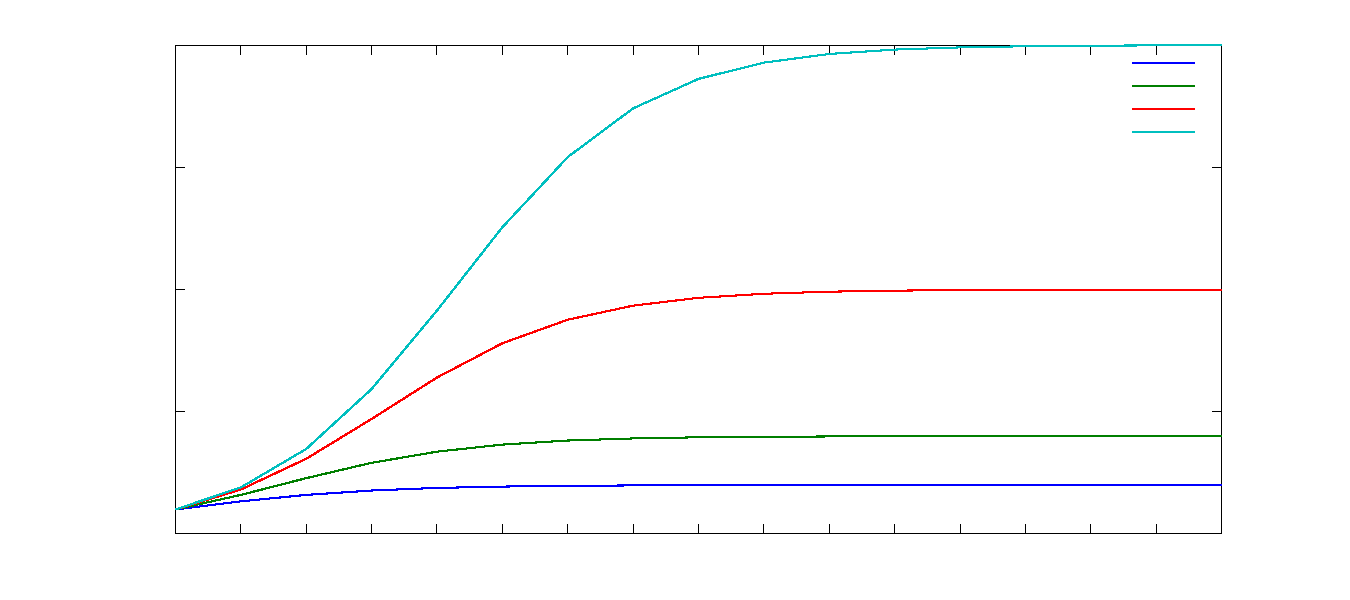
\includegraphics{amdahl}}%
    \gplfronttext
  \end{picture}%
\endgroup
